\subsection{Current Sources}\label{sec:currentsources}
The final stage of the power DAC are the current sources. They provide a differential output through a 50$\Omega$ resistor. This setup is shown in Fig. \ref(figure:Current_sources).
\begin{figure}
\begin{center}
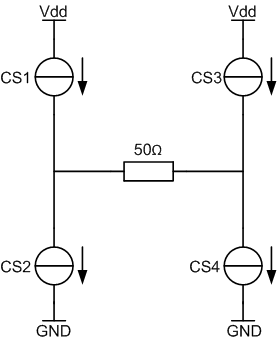
\includegraphics[width=10cm]{Current_sources.png}
\caption{The final stage of the power DAC: The current sources which will provide the differential output through the resistor.}
\label{figure:Current_sources}
\end{center}
\end{figure}
Due to the local oscillator, the current will alternate between $V_{dd} \rightarrow CS1 \rightarrow CS4 \rigtharrow GND$ (see Fig.\ref{figure:CS1CS4}) and $V_{dd} \rightarrow CS3 \rightarrow CS2 \rigtharrow GND$ (see Fig.\ref{figureCS3CS2}). 
\begin{figure}
\begin{center}
\begin{subfigure}{0.5\textwidth}
\begin{center}
\includegraphics[width=0.4\linewidth]{Current_sources1.png}
\caption{One current-steered cycle.}
\label{fig:CS1CS4}
\end{center}
\end{subfigure}
\begin{subfigure}{0.5\textwidth}
\begin{center}
\includegraphics[width=0.4\linewidth]{Current_sources2.png}
\caption{The other current-steered cycle.}
\label{fig:CS3CS2}
\end{center}
\end{subfigure}
The first design parameters are the voltage supply and which switching devices are to be used. Because the DAC should be able to produce 50mA through a 50$\Omega$ resistor, the maximum voltage drop will be 2.5V. This already cancels out lower voltage supplies such as 1.2V and 2.5V. The resulting options are 3.3V and 5V. Because the stage consist of two current sources, the voltage headroom will be very limited in the 3.3V voltage supply. Therefor a 5V supply will be used as $V_{dd}$. This, along with the high switching speeds, limits the switching devices to the thick-oxide CMOS technology.\\
Because thick-oxide CMOS technology has been chosen, the width and length of the CMOS are the only parameters. The most straightforward design method subscribes that the CMOS should always be in saturation so that the current through the CMOS is independent of the drain-source voltage of the CMOS. Therefor Eq.\ref{eq:Overdrive} should be valid whatever the drain-source voltage.
\begin{equation}[ht!]
\begin{center}
V_{DS} > V_{TH} + V_{GS}
\label{eq:Overdrive}
\end{center}
\end{equation}
The drain-source voltage of the NMOS is minimal when the current through the resistor is maximal. This results in a minimum drain-source voltage of 1.25V. Because Eq.\ref{eq:Overdrive} should be valid independent of the output, the maximum gate-source provided by the level shifter should be 1.95V, because the threshold voltage of the thick-oxide CMOS is 0.7V. Along with Eq.\ref{eq:Drain current}, this would provide the perfect current sources.
\begin{equation}[ht!]
\begin{center}
I_D = \frac{1}{2}\mu_n C_{ox}\frac{W}{L}(V_{GS}-V_{TH})^2(1+\lambda V_{DS})
\ref{eq:Drain current}
\end{center}
\end{equation}
The main disadvantage of this straightforward approach is that this leads to significant speed restrictions. The small overdrive voltage, $V_{DS}-V_{TH}$, will require large width and thus large input capacitances. Due to the large input capacitance the level shifter will not be able to drive the gate-source voltage to the appropriate voltage level. So for the level shifter to work properly, the width of the NMOS should be increased. This will lead to a signal dependent error in the current. This can be seen from the FFT of the total system, the IMD3-level will increase due to this signal-dependence. So the trade-off will be to maximize the width of the NMOS, and therefor also the PMOS, while keeping the level-shifter in its desired working area.\\
Another aspect which has not been accounted for, is the channel-length modulation. As can be seen from Eq.\ref{eq:Drain current}, the channel length modulation depend on both intrinsic parameters, $\lambda$, and extrinsic parameters, $V_{DS}$. The drain-source voltage is signal dependent. Each active stage of NMOS, will decrease the drain-source voltage. Because the intrinsic parameter $\lambda$ is inverse proportional to the length of the NMOS, the length of the NMOS can be also be decreased so that the current delivered by the NMOS does not alter for different signals.

The next paper will contain information about the IMD3 - width trade-off and corresponding simulations. It will also contain viable designs.  